\documentclass[11pt]{article}
\newcommand{\MODULETAG}{Module 1\,\textbar\,Foundations}
% ===== Toro Resource Estimation Course - shared PDF preamble =====
\usepackage[a4paper,margin=2.4cm,headsep=14pt]{geometry}
\usepackage{amsmath,amssymb}
\usepackage{lmodern}
\usepackage[T1]{fontenc}
\usepackage[utf8]{inputenc}
\usepackage{microtype}
\usepackage{graphicx}
\usepackage{booktabs}
\usepackage{array}
\usepackage{enumitem}
\usepackage{xcolor}
\usepackage{titlesec}
\usepackage{fancyhdr}
\usepackage[most]{tcolorbox}
\usepackage{listings}
\usepackage{caption}
\usepackage[hidelinks]{hyperref}

% ---- palette ----
\definecolor{navy}{HTML}{1F2A44}
\definecolor{navy2}{HTML}{2B3A5C}
\definecolor{bronze}{HTML}{C8702D}
\definecolor{bronzed}{HTML}{A85A1F}
\definecolor{teal}{HTML}{2A7D8C}
\definecolor{tealw}{HTML}{ECF4F5}
\definecolor{ink}{HTML}{26303F}
\definecolor{paper2}{HTML}{F3EDE1}
\definecolor{line}{HTML}{D8D4CB}
\definecolor{codebg}{HTML}{1C2433}
\definecolor{good}{HTML}{3F7D5A}
\definecolor{warn}{HTML}{B4451F}

\color{ink}
\setlength{\parindent}{0pt}
\setlength{\parskip}{6pt}
\linespread{1.06}

% ---- section styling ----
\titleformat{\section}{\Large\bfseries\color{navy}}{\thesection}{0.6em}{}
\titleformat{\subsection}{\large\bfseries\color{navy2}}{\thesubsection}{0.6em}{}
\titleformat{\subsubsection}{\normalsize\bfseries\color{bronzed}}{}{0em}{}
\titlespacing{\section}{0pt}{16pt}{6pt}
\titlespacing{\subsection}{0pt}{12pt}{4pt}

% ---- header / footer ----
\pagestyle{fancy}
\fancyhf{}
\renewcommand{\headrulewidth}{0.4pt}
\renewcommand{\footrulewidth}{0pt}
\fancyhead[L]{\footnotesize\color{navy2}\MODULETAG}
\fancyhead[R]{\footnotesize\color{navy2}Toro Tin Project\,\textbar\,ANRML26-137}
\fancyfoot[C]{\footnotesize\color{navy2}\thepage}

% ---- callout boxes ----
\newtcolorbox{keybox}[1][Key concept]{breakable,enhanced,
  colback=paper2,colframe=bronze,boxrule=0pt,leftrule=4pt,
  arc=2pt,left=10pt,right=10pt,top=8pt,bottom=8pt,
  fonttitle=\bfseries\sffamily\small\color{bronzed},title={#1}}
\newtcolorbox{torobox}[1][Toro application]{breakable,enhanced,
  colback=navy!6,colframe=navy,boxrule=0pt,leftrule=4pt,
  arc=2pt,left=10pt,right=10pt,top=8pt,bottom=8pt,
  fonttitle=\bfseries\sffamily\small\color{navy},title={#1}}
\newtcolorbox{pitbox}[1][Common pitfall]{breakable,enhanced,
  colback=warn!7,colframe=warn,boxrule=0pt,leftrule=4pt,
  arc=2pt,left=10pt,right=10pt,top=8pt,bottom=8pt,
  fonttitle=\bfseries\sffamily\small\color{warn},title={#1}}
\newtcolorbox{notebox}[1][Note]{breakable,enhanced,
  colback=tealw,colframe=teal,boxrule=0pt,leftrule=4pt,
  arc=2pt,left=10pt,right=10pt,top=8pt,bottom=8pt,
  fonttitle=\bfseries\sffamily\small\color{teal},title={#1}}
\newtcolorbox{defbox}[1][Definition]{breakable,enhanced,
  colback=good!7,colframe=good,boxrule=0pt,leftrule=4pt,
  arc=2pt,left=10pt,right=10pt,top=8pt,bottom=8pt,
  fonttitle=\bfseries\sffamily\small\color{good},title={#1}}
\newtcolorbox{objbox}{enhanced,colback=navy,colframe=navy,
  arc=3pt,left=12pt,right=12pt,top=10pt,bottom=10pt,
  coltext=white}

% ---- python code ----
\lstdefinestyle{py}{language=Python,
  basicstyle=\footnotesize\ttfamily\color{white},
  keywordstyle=\color{bronze},commentstyle=\color{line},
  stringstyle=\color{teal!60!white},backgroundcolor=\color{codebg},
  numberstyle=\tiny\color{line},showstringspaces=false,
  breaklines=true,frame=single,framerule=0pt,
  rulecolor=\color{codebg},xleftmargin=8pt,xrightmargin=4pt,
  aboveskip=10pt,belowskip=6pt,framexleftmargin=8pt,
  framexrightmargin=8pt,framextopmargin=6pt,framexbottommargin=6pt}
\lstset{style=py}

% ---- equation box ----
\newtcolorbox{eqbox}{enhanced,colback=white,colframe=line,
  boxrule=0.6pt,arc=2pt,left=8pt,right=8pt,top=4pt,bottom=4pt,
  before skip=10pt,after skip=10pt}

% ---- captions ----
\captionsetup{font={small,it},labelfont={bf,color=navy},labelsep=endash}

% ---- module title macro ----
\newcommand{\moduletitle}[3]{%
  {\sffamily\bfseries\footnotesize\color{bronze}\MakeUppercase{#1}\par}
  \vspace{2pt}
  {\sffamily\bfseries\LARGE\color{navy}#2\par}
  \vspace{3pt}
  {\small\itshape\color{navy2}#3\par}
  \vspace{4pt}{\color{line}\hrule height 1.5pt}\vspace{12pt}}

\begin{document}

\moduletitle{Module 1 of 6}{Foundations: Resources, Reserves and the
Reporting Codes}{Resource Estimation \& Geostatistics --- a technical
training course built on the live ANRML26-137 / EL-046017 datasets}

Before a single variogram is fitted, you must know exactly what you are
trying to produce, what word you are allowed to put on it, and who is
legally accountable for it. This module installs that framework.
Everything in Modules 2 to 6 is machinery in service of the definitions
you learn here.

\begin{objbox}
{\sffamily\bfseries\color{bronze}LEARNING OBJECTIVES}
\begin{itemize}[leftmargin=14pt,itemsep=2pt]
\item State precisely what a Mineral Resource and an Ore Reserve are, and
the test that separates them.
\item Explain the CRIRSCO family of codes and the legal role of the
Competent or Qualified Person.
\item Place an estimate into the Inferred--Indicated--Measured framework
and justify the category against evidence.
\item Enumerate the modifying factors and explain how they convert a
Resource into a Reserve.
\item Define an Exploration Target and explain why Toro currently is one.
\end{itemize}
\end{objbox}

\section{The question resource estimation answers}

A mineral deposit is, commercially, a single quantity of money buried in
a single volume of rock. The whole of resource estimation exists to
answer one question precisely enough that capital will move on the
answer.

\begin{keybox}[The central question]
For a defined volume of ground: \textbf{how many tonnes are there, at
what average grade, and with what level of confidence?} The third clause
is not optional. An estimate without a stated confidence is not a
resource estimate --- it is a guess with decimal places.
\end{keybox}

Tonnes and grade are the two estimated quantities; confidence is the
meta-statement about how far they can be trusted. Geostatistics
(Modules 4--5) is the mathematics of that third clause. The two estimated
quantities combine into the number that matters, contained metal:

\begin{eqbox}
\[ M = T \times \bar{g} \tag{1.1}\]
\end{eqbox}

Grade carries units that must be handled with discipline. The Toro
laboratory reports tin as the oxide SnO$_2$ in weight per cent; metal
accounting and contracts use the element Sn. The conversion is a fixed
stoichiometric factor:

\begin{eqbox}
\[ \mathrm{Sn} = \mathrm{SnO_2}\times\frac{M_{\mathrm{Sn}}}{M_{\mathrm{SnO_2}}}
   = \mathrm{SnO_2}\times\frac{118.71}{150.71}
   = 0.7877\;\mathrm{SnO_2} \tag{1.2}\]
\end{eqbox}

A reported 6.04\% SnO$_2$ in Toro pit DBP-002 is 4.76\% Sn. Mixing the
two is one of the most common and most expensive reporting errors in
tin projects.

\subsection{The exploration value chain}

A resource estimate is one station on a chain running from a geological
idea to a financed mine. Each transition is a \emph{decision gate}: if
results do not justify the next, larger tranche of capital, the project
is downgraded, deferred or relinquished.

\begin{center}\small
\begin{tabular}{@{}p{4.6cm}p{4.6cm}p{4.6cm}@{}}
\toprule
\textbf{Stage} & \textbf{Output} & \textbf{Toro status (May 2026)}\\
\midrule
Desktop study & Prospectivity model, targets & Substantially complete\\
Reconnaissance & Field-confirmed anomalies & Complete: 47 XRD, 40 XRF\\
Systematic pitting & Stratigraphy, Exploration Target & In progress\\
Resource drilling & Drillhole database & 13 priority collars defined\\
\textbf{Resource estimate} & Classified Resource statement & Destination
of this course\\
Studies / Reserve & Feasibility, an Ore Reserve & Future\\
\bottomrule
\end{tabular}
\end{center}

\section{Why there are codes at all}

Public reporting of mineral assets is regulated because the history of
not regulating it is a history of fraud. The \textbf{Poseidon bubble}
(Australia, 1969--70) drove a nickel stock from under a dollar to GBP 280
and back on unregulated reporting. The \textbf{Bre-X fraud} (Busang,
1995--97) salted drill core with placer gold, claimed a fictitious
70-million-ounce deposit, and erased roughly USD 6 billion of value.

\begin{defbox}[The CRIRSCO family]
The Committee for Mineral Reserves International Reporting Standards
maintains an international \emph{template}. National codes implement it:
\textbf{JORC} (Australasia), \textbf{NI 43-101} with the CIM Definition
Standards (Canada), \textbf{SAMREC} (South Africa), \textbf{PERC}
(Europe). They share one architecture, so a Resource is portable across
exchanges. Nigeria has no domestic code, so a Toro estimate intended to
raise capital will be reported under JORC or NI 43-101.
\end{defbox}

Three principles run through every code: \textbf{transparency} (the
reader is given enough information not to be misled), \textbf{materiality}
(all information a reasonable investor would require), and
\textbf{competence} (a named, accountable signatory).

\begin{keybox}[The Competent / Qualified Person]
A \textbf{Competent Person} (JORC) or \textbf{Qualified Person}
(NI 43-101) takes personal, legal responsibility for the estimate. They
must hold membership of a Recognised Professional Organisation and have
at least five years of experience \emph{relevant to the style of
mineralisation under consideration}. That phrase matters for Toro:
hard-rock gold experience does not qualify a person to sign an alluvial
tin placer. COMEG registration and NMGS membership are the route to this
status in the Nigerian context.
\end{keybox}

\section{Mineral Resource versus Ore Reserve}

\begin{defbox}[Mineral Resource]
A concentration of material of economic interest in or on the Earth's
crust in such form, grade and quantity that there are \emph{reasonable
prospects for eventual economic extraction}. Defined on the basis of
geological evidence and knowledge.
\end{defbox}

\begin{defbox}[Ore Reserve]
The economically mineable part of a Measured or Indicated Mineral
Resource, demonstrated by at least a Pre-Feasibility Study that has
applied the modifying factors.
\end{defbox}

Three consequences follow. A \textbf{Resource is geological; a Reserve is
engineering plus economics}. \textbf{Resources are not a subset of
Reserves --- it is the reverse}: a Reserve is carved from the Measured
and Indicated parts of a Resource, and an Inferred Resource can never
become a Reserve without further drilling. And \textbf{``reasonable
prospects for eventual economic extraction'' (RPEEE) is a real,
enforceable test}: you demonstrate it by constraining the estimate inside
a conceptual mining envelope at a reasonable price and cut-off. Material
that cannot sit within a plausible mining shape is not a Resource.

\section{The classification framework}

Within a Mineral Resource, confidence is graded into three categories ---
each a statement about how much geology has been \emph{demonstrated}
rather than \emph{assumed}.

\begin{center}\small
\begin{tabular}{@{}p{2.4cm}p{12cm}@{}}
\toprule
\textbf{Inferred} & Estimated on limited evidence; geological and grade
continuity \emph{implied but not verified}. Cannot be converted to a
Reserve.\\[3pt]
\textbf{Indicated} & Estimated with enough confidence to \emph{reasonably
assume} continuity. Supports a Pre-Feasibility Study; converts to a
\textbf{Probable} Reserve.\\[3pt]
\textbf{Measured} & Estimated with enough confidence to \emph{confirm}
continuity. Supports a Feasibility Study; converts to a \textbf{Proven}
Reserve.\\
\bottomrule
\end{tabular}
\end{center}

The codes express classification as a two-dimensional structure: one axis
is geological confidence (raised by drilling and sampling), the other is
the modifying factors (applied by study engineers). An Inferred Resource
has no path straight to a Reserve --- it must first be upgraded.

\begin{pitbox}
It is tempting to think the categories are defined by drill spacing alone
(``50 m equals Measured''). They are not. Drill spacing is evidence, but
the category is a \emph{judgement about continuity} made by the Competent
Person, supported by variography (Module 4), geological understanding and
QAQC. Two deposits at identical spacing can warrant different categories.
\end{pitbox}

\section{The modifying factors}

The modifying factors convert a geological Resource into an economically
mineable Reserve. A code-compliant study addresses each one explicitly:
\textbf{mining} (can it be mined, at what dilution and recovery),
\textbf{processing} (can the metal be liberated --- cassiterite is
gravity-recoverable, columbite needs magnetic separation),
\textbf{economic} (does it pay at a realistic long-term tin price),
\textbf{marketing} (concentrate specification and penalties),
\textbf{infrastructure}, \textbf{legal/tenure}, \textbf{environmental},
and \textbf{social/governmental}. For the Toro alluvial target one factor
demands early attention: the wash gravels are already mined by artisanal
operators --- simultaneously a confirmation of grade continuity and a
serious social and tenure factor.

\section{The Exploration Target --- and why Toro is one}

\begin{defbox}[Exploration Target]
A statement of the \emph{exploration potential} of a deposit, expressed
as \textbf{ranges} of tonnage and grade. It must be clearly labelled as
conceptual, state that there has been insufficient exploration to
estimate a Mineral Resource, and not be capable of being misread as one.
\end{defbox}

\begin{torobox}[Where Toro stands today]
The current Toro grade data is a reconnaissance dataset: 40 XRF analyses
collapsing to roughly \textbf{26 distinct pit locations} once laboratory
mineral-separation fractions are removed (Module 2). Those pits spread
across three drainages over several kilometres. Two facts follow. First,
the sampling density cannot support an assumption of grade continuity at
any mining scale --- so no category above Exploration Target is
defensible. Second, the panned-concentrate sampling medium does not by
itself give an in-situ g/m$^3$ grade. Toro is an Exploration Target
because the data type and density make it one, and only drilling and
systematic pitting can change that.
\end{torobox}

\section{The Achmmach benchmark}

Atlantic Tin's Achmmach project in Morocco reached, after roughly 18
years, a Measured and Indicated Resource of \textbf{22.4 Mt at 0.70\%
Sn} (about 156,000 t contained tin) and Proven and Probable Reserves of
\textbf{7.0 Mt at 0.82\% Sn} (about 58,000 t contained tin). The Resource
is the larger, geologically defined quantity; the Reserve is the smaller
part a feasibility study showed could be mined, at slightly higher grade
because marginal material fell below cut-off. That is the
Resource-to-Reserve relationship in real numbers. Toro's task over the
next five to seven years is to earn the right to write a comparable pair
of lines.

\begin{figure}[h]\centering
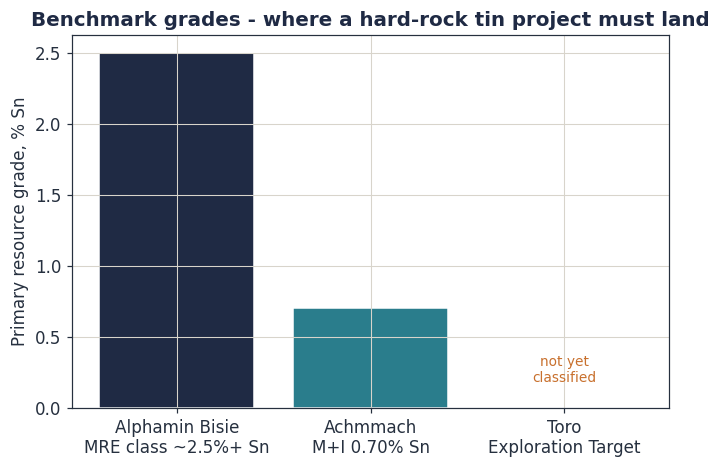
\includegraphics[width=0.78\textwidth]{../assets/figures/fig_benchmark.png}
\caption{Where a hard-rock tin project must land. Toro's primary target
has no classified grade yet --- it is an Exploration Target.}
\end{figure}

\vspace{4pt}
{\color{line}\hrule}
\vspace{4pt}
{\small\itshape Module 1 of the Toro Resource Estimation \& Geostatistics
course. Next: Module 2, Sampling, Data and Database Integrity.}

\end{document}
